Per soluzione si intende un sistema omogeneo di due o più componenti. Nei nostri studi ci limiteremo al caso di soluzioni formate da due componenti, che etichetteremo con \textbf{solvente} e \textbf{soluto}.

A priori, l'unico criterio che abbiamo per fare questa distinzione quando si hanno due liquidi totalmente miscibili è vedere quale dei due sia più abbondante: quello più abbondante sarà il solvente, quello meno abbondante il soluto. Se quindi ad esempio avessimo una soluzione acqua-alcol, tra i due il solvente sarà quello che in proporzione è presente in percentuale maggiore.

\subsection{Alcune distinzioni e primi esempi}

\begin{figure}[htp]
    \centering
    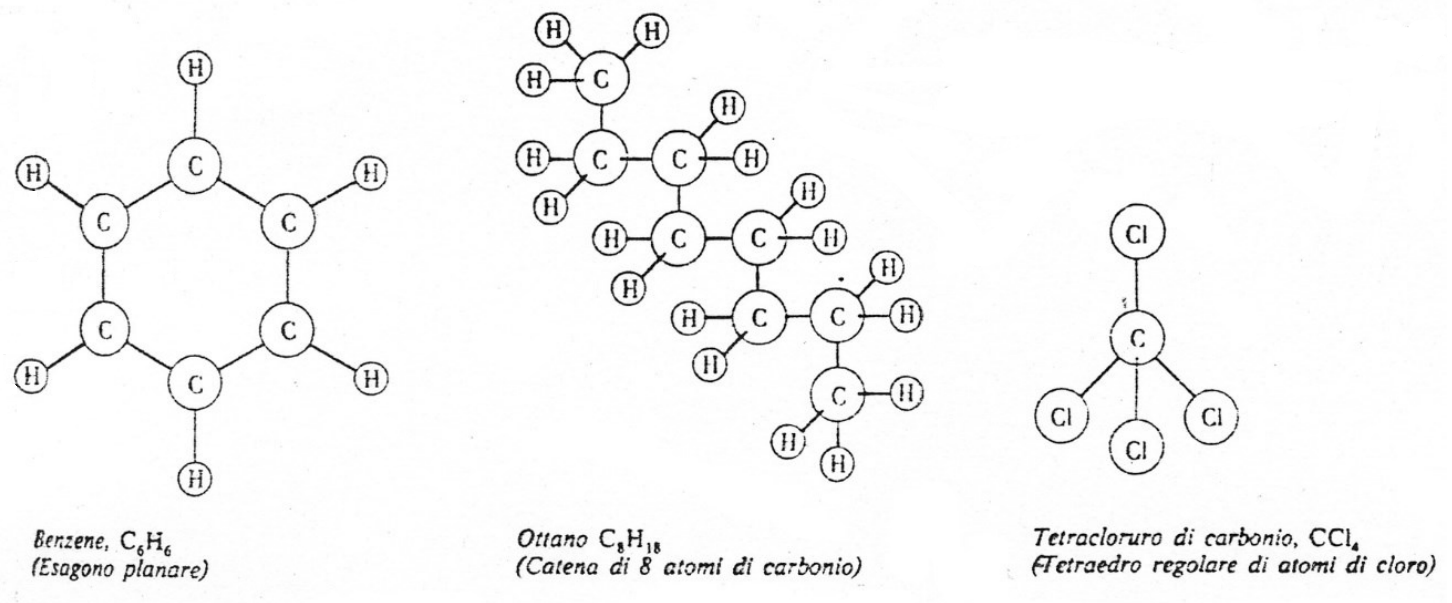
\includegraphics[width=11cm]{immagini/molecole_non_polari.png}
\end{figure}

L'acqua ha una struttura dipolare, cioè ha un forte momento di dipolo, caratteristica fondamentale per le sue proprietà. Al contrario, molecole come il benzene C$_6$H$_6$, l'ottano C$_8$H$_8$ e il tetracloruro di carbonio CCl$_4$ non mostrano momento di dipolo.

\E chiaro quindi che possiamo distinguere molecole polari e non polari. Sono molecole polari:

\begin{itemize}
    \item L'acqua;
    \item L'alcol metilico (o metanolo) CH$_3$OH, perché c'è una buona differenza di elettronegatività tra ossigeno ed idrogeno, dovuta al fatto che l'ossigeno è molto elettronegativo, conferendo una certa polarità alla molecola;
    \item L'ammoniaca perché non è planare (a differenza del BF$_3$).
\end{itemize}

\begin{figure}[htp]
    \centering
    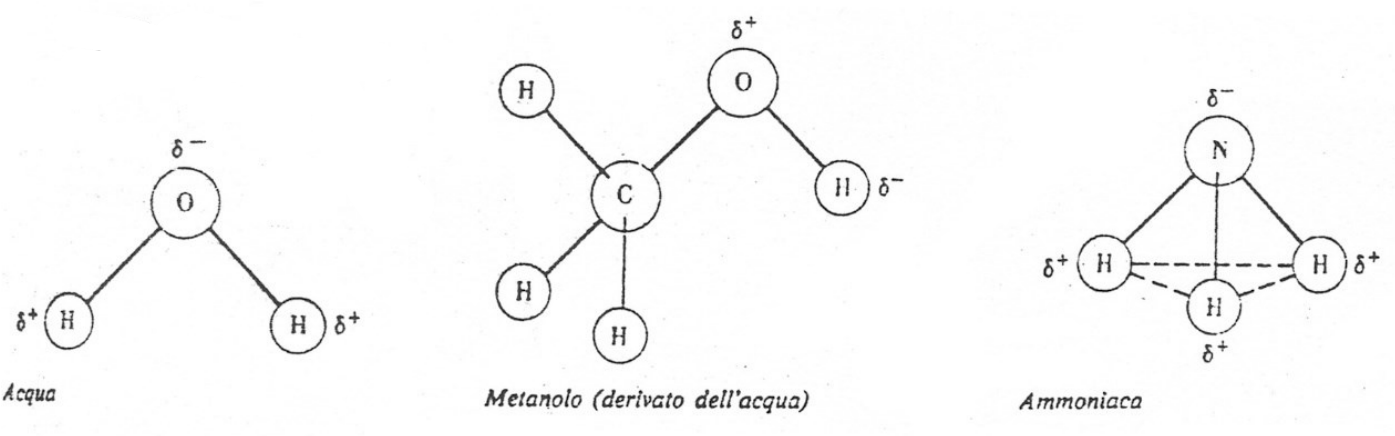
\includegraphics[width=11cm]{immagini/molecole_polari}
\end{figure}

La polarità determinerà le proprietà di solvatazione, che il fenomeno per cui un solvente scioglie un soluto.

\vspace{0.2cm}Si hanno diversi tipi di soluzione:

\vspace{0.2cm}$\bullet$ Soluzioni gassose
\begin{itemize}
    \item[$-$]Gas-gas. Tutti i gas formano soluzioni. Se avessimo due gas a comportamento ideale ognuno si comporterebbe come se fosse l'unico presente. Se questa idealità viene a mancare parliamo di soluzione gassosa.
\end{itemize}

$\bullet$ Soluzioni liquide
\begin{itemize}
    \item[$-$]Liquido-liquido (es. acqua-alcol);
    \item[$-$]Gas-liquido (es. i pesci respirano ossigeno, il quale è sciolto nelle acque dei fiumi, laghi e mari; le bevande gassose: anidride carbonica in acqua)
    \item[$-$]Solido-liquido (es. cloruro di sodio in acqua, zucchero in acqua) 
\end{itemize}
\vspace{0.2cm}$\bullet$ Soluzioni solide
\begin{itemize}
    \item[$-$]Solido-solido, ad es. leghe di metalli diversi. Ne è un esempio il rubino, che è formato dall'ossido di alluminio $\rm Al_2O_3$ contenente impurezze di ossido di cromo $\rm Cr_2O_3$.
\end{itemize}
Concentreremo l'attenzione sulle soluzioni liquide.

Ragioniamo sul fenomeno della formazione della soluzione. Cosa significa dissolvere qualcosa?

\vspace{0.2cm}\textbf{Es.1 Alcol metilico (metanolo) $\boldsymbol{\rm CH_3OH}$ in acqua}

\begin{figure}[htp]
    \centering
    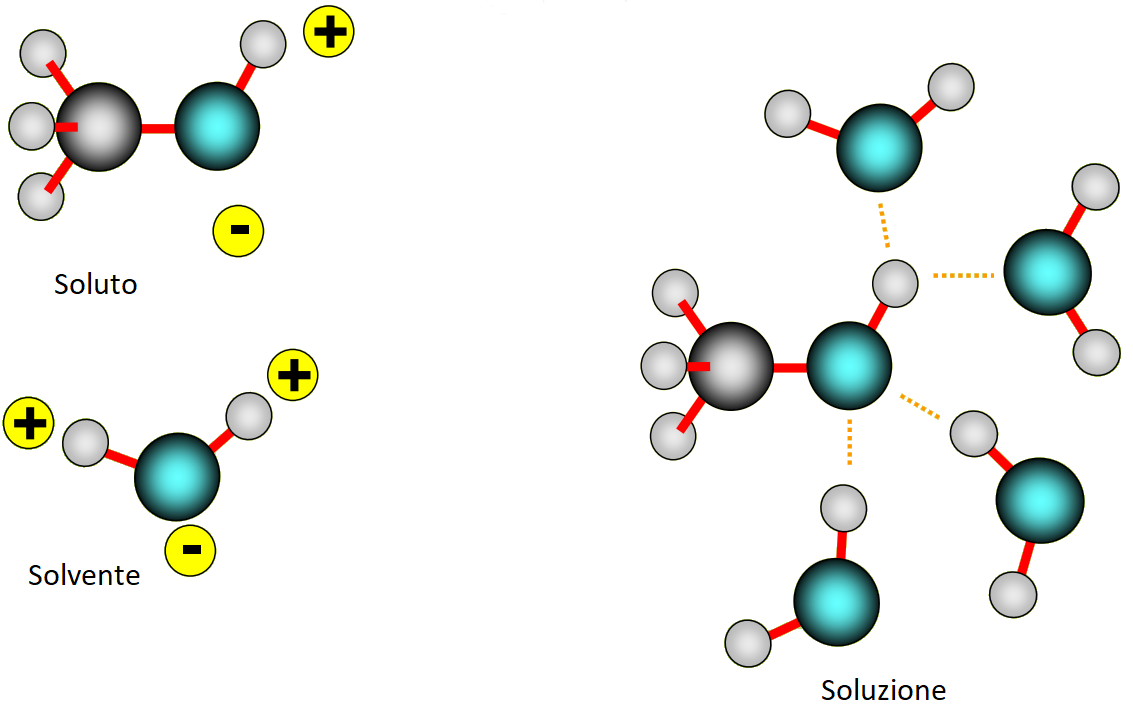
\includegraphics[width=9cm]{immagini/acido_acetico.png}
\end{figure}

Nella molecola CH$_3$OH troviamo polarità nel legame ossigeno-idrogeno. Se mettiamo tale molecola in acqua (attenzione! Stiamo considerando l'acqua come solvente e il metanolo come soluto, quindi esso sarà meno abbondante), la quale è una molecola fortemente polare che mostra carica negativa sull'ossigeno e carica positiva sui due atomi di idrogeno, tra i due tipi di molecole si realizzeranno delle interazioni dettate dalla diversa carica o più precisamente dalla diversa polarità (si tratta di cariche parziali): gli idrogeni dell'acqua si orientano verso l'ossigeno del metanolo, mentre l'idrogeno del metanolo reagirà con gli ossigeni della molecola dell'acqua.

Si realizza così nella soluzione un sistema esteso di interazioni. Dunque il fenomeno di soluzione non è un semplice mescolamento che non comporta interazioni fra le specie considerate: in esso vediamo formarsi nuove interazioni tra soluto e solvente.

Però soltanto nell'acqua appaiono già i legami ad idrogeno: l'ossigeno di una molecola d'acqua interagirà con l'idrogeno di un'altra molecola d'acqua. Quindi pur avendo come unico componente l'acqua liquida esistono già forti interazioni dovute alla forte differenza di elettronegatività tra ossigeno e idrogeno. Interazioni simili si realizzano tra metanolo e acqua.

\vspace{0.2cm} Consideriamo ora un cristallo di cloruro di sodio Na$^+$Cl$^-$

\begin{figure}[htp]
    \centering
    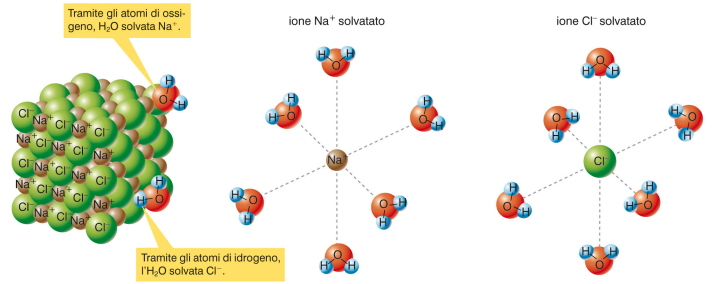
\includegraphics[width=12cm]{immagini/solvatazione_cloruro_di_sodio.png}
\end{figure}

In esso abbiamo ioni che occupano precise posizioni reticolari. La forza che tiene insieme questi ioni può essere descritta approssimativamente dalla legge di Coulomb:
$$\displaystyle F= \frac{1}{4 \pi \varepsilon} \cdot \frac{q_1 \, q_2}{r^2}$$
dove $\varepsilon$ è la costante dielettrica che nel vuoto vale $8.8544 \cdot 10^{-12}\;C^2/Nm^2$, nell'aria vale 1 e nell'acqua vale 80. Ecco perché l'acqua riesce a sgretolare, cioè a portare in soluzione, anche cristalli di cloruro di sodio: essa attacca singolarmente gli ioni, portandoli in soluzione. Ciò che avviene nel processo di solvatazione è che più molecole d'acqua circondano gli ioni uno ad uno, li solvatano e lo portano in soluzione. Il numero di molecole d'acqua che circonda ogni ione è casuale.

L'aver ottenuto una soluzione significa che se avevamo un cristallo di cloruro di sodio e delle molecole di acqua che lo hanno circondato, ogni singolo ione è stato poi circondato da molecole di acqua.

Nel caso dello ione cloruro sono gli atomi di idrogeno ad essere rivolti verso di esso, mentre per lo ione sodio sono gli ossigeni a vertere verso di esso, questo perché gli atomi di idrogeno hanno parziale carica positiva e quelli di ossigeno parziale carica negativa.

Lo ione sodio Na$^+$ è così piccolo perché ha perso un elettrone e ha assunto la configurazione elettronica del gas nobile che lo precede, ossia il neon, mentre lo ione cloruro Cl$^-$ è così grosso perché ha acquistato un elettrone, assumendo la configurazione elettronica del gas nobile che lo segue, ossia l'argon.

\vspace{0.2cm}Abbiamo visto che un cristallo ionico viene sciolto da una molecola polare. In generale vale la seguente regola: "\textit{il simile scioglie il simile}", ossia se avessimo una specie non polare, ad esempio l'olio, questa non si discioglierebbe in acqua. Pertanto per sciogliere una sostanza non polare è opportuno usare un solvente non polare. Ad esempio il CCl$_4$ è un buon solvente apolare, quindi non può sciogliere il cloruro di sodio.

\subsection{Energie in gioco}

Consideriamo ancora la solubilizzazione del cloruro di sodio in acqua. Se volessimo rappresentare da un punto di vista energetico questo fenomeno, quali sono le energie in gioco?

\hspace{-0.2cm}\begin{figure}[H]
    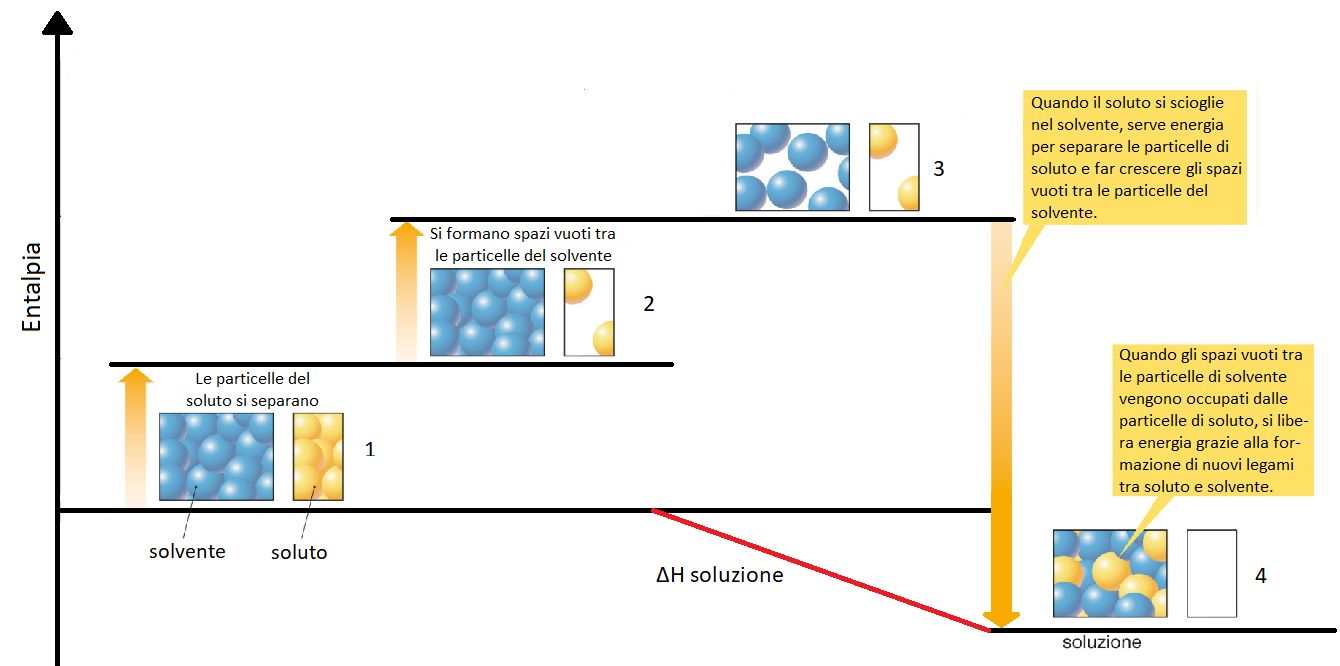
\includegraphics[width=15.6cm]{immagini/entalpia_soluzioni.png}
\end{figure}

Immaginiamo di avere, separati, il solvente ed il soluto.

La prima operazione da fare è allontanare le varie particelle di soluto. Abbiamo visto, studiando il legame ionico, che esiste l'energia reticolare, cioè l'energia che si libera quando si forma un reticolo, ossia quando un certo numero di ioni gassosi collassa e dà il solido. Se vogliamo riallontanare questi ioni dobbiamo spendere esattamente l'energia reticolare. Ne segue che il primo gradino in energia è dato dall'energia reticolare del cristallo.

Se però vogliamo ottenere una soluzione dobbiamo poi allontanare fra loro anche le particelle di solvente. Nel caso specifico in cui il solvente sia l'acqua, dovremo rompere i legami ad idrogeno fornendo l'energia che costituisce il secondo gradino.

A questo punto abbiamo separato sia le particelle del solvente che quelle del soluto. Quando esse si mescolano c'è un crollo di energia: si arriva ad un livello energetico più negativo di quello di partenza, ossia c'è un guadagno in energia e infatti il sistema libera calore. Avremo quindi una soluzione stabile.

Va ricordato che per convenzione l'energia ceduta all'ambiente è negativa, mentre quella assorbita dal sistema è positiva. Pertanto, essendo una reazione esotermica, avremo un $\Delta$H negativo, che rappresenta l'energia ceduta all'ambiente.
